\documentclass[12pt,twoside]{article}
\usepackage[a4paper,top=3cm, bottom=3cm, left=2cm, right=2cm]{geometry}
\usepackage{graphicx}
\usepackage[superscript,biblabel]{cite}
\usepackage{authblk}
\usepackage{amsmath, amsthm, amssymb, amsfonts}
\usepackage{bbm}
\usepackage{float}
\usepackage[table]{xcolor}% http://ctan.org/pkg/xcolor
\usepackage[ddmmyyyy]{datetime}

\linespread{1.1}
\paperwidth=210mm
\parindent=0pt


\begin{document}


\begin{center}
{\LARGE \texttt{Permar} - a suite of analysis routines for the \texttt{Lare3d} code}

Val Aslanyan -- 26/12/22
\end{center}

{\large \textbf{Summary}}

\vspace{1mm}

$\quad\quad$\textit{\textbf{LARE}S \textbf{PERMAR}INI}: Roman guardian deities of seafarers

\vspace{1mm}

This package contains native \texttt{Python3} routines to read, process and display outputs from the \texttt{Lare3d} code. In particular, the \texttt{SDF} file format of the Centre for Fusion Space and Astrophysics (CFSA) at the University of Warwick (as opposed to a completely different and more widespread scientific SDF file format) can be read using a single \texttt{Python} function without the need for external routines.

There is also an extension to the \texttt{Lare3d} code itself to output the velocity at \textit{e.g.} the bottom boundary every timestep, thereby allowing the ``footpoints'' of magnetic field lines to be accurately tracked throughout the simulation. Higher level quantities such as the squashing factor $Q$ and the connectivity of magnetic field lines can also be calculated.

The package is written mostly in \texttt{Python} version $\geq 3.7$, with additional high-performance routines in \texttt{Fortran 90}.


\vspace{4mm}
{\large \textbf{Installing and using \texttt{Permar}}}

Clone the \texttt{Permar} git repository
You will see the main \texttt{Permar\_Functions\_Python.py} file containing the main processing routines - this should be kept once, pulled from the repository as required and probably not modified. Alongside are smaller scripts which you will probably want to copy and paste into multiple folders with \texttt{Lare} runs as required and modify heavily.

\vspace{2mm}

Near the top of every one of the smaller scripts is the following preamble, which will load the prerequisite libraries and the \texttt{Permar} routines themselves if the string \texttt{\textquotesingle /Change/This/Path\textquotesingle} is set to the location of \texttt{Permar\_Functions\_Python.py}:

$\quad\quad$\texttt{import sys}

$\quad\quad$\texttt{sys.path[:0]=[\textquotesingle /Change/This/Path\textquotesingle ]}

$\quad\quad$\texttt{from Permar\_Functions\_Python import *}

\vspace{2mm}

The routines and scripts should be easy to follow for anyone familiar with \texttt{Python}. Take a look at \texttt{ReadLare3d.py} as a starting point. There is a function call to read 

$\quad\quad$\texttt{lare3d\_file\_properties,lare3d\_blocks=read\_cfsasdf\_file(lare3d\_filename)}

Normalizing constants are read from the \texttt{lare3d.dat} file as follows:

$\quad\quad$\texttt{lare3d\_dat=read\_lare3d\_dat(lare3d\_datfilename)}

Once loaded, a specific quantity can be extracted from the blocks with \texttt{quantity\_from\_blocks} for a generic grid/quantity combination or \texttt{regularize\_Bfield}, which will return the magnetic field on a single cell-centered grid (normally, each component is stored by \texttt{Lare3d} at a different cell edge location).

\vspace{2mm}

If memory becomes an issue, for example if a single array is $>10$GB, the following function call will return a single quantity as economically as possible,

$\quad\quad$\texttt{time,grid\_x,grid\_y,grid\_z,data=read\_cfsasdf\_file\_lean(filename,target)}

where \texttt{target} is a string specifying the quantity.

\vspace{2mm}
\newpage

The following widespread \texttt{Python} modules are used in the package:

\vspace{-3mm}

\begin{itemize}
\setlength\itemsep{-2mm}
  \item \textbf{numpy} [mandatory]
  \item \textbf{matplotlib} [2D plotting]
  \item \textbf{mayavi} [3D plotting]
\end{itemize}

\vspace{-2mm}

To install \texttt{Python} modules, type the following into a terminal:

$\quad\quad$\texttt{pip3 install [module] --user}


\vspace{8mm}
{\large \textbf{What is not included in the package}}

\begin{itemize}
\setlength\itemsep{-2mm}

  \item \textbf{ffmpeg} - required for movies; this is open source and can be installed straightforwardly on Linux/Windows
\vspace{2mm}

  \item Base version of \texttt{Lare3d} - this can be cloned from 

\vspace{-3mm}
https://github.com/Warwick-Plasma/Lare3d
\vspace{2mm}

  \item Modified version of \texttt{Lare3d} to output surface velocity - can be obtained from me on request

\vspace{2mm}
  \item Base version of \texttt{QSL Squasher} - this can be cloned from 

\vspace{-3mm}
https://bitbucket.org/tassev/qsl\_squasher/src/hg/
\vspace{2mm}

  \item Modified version of \texttt{QSL Squasher} which writes its result to a structured file - can be obtained from me on request
\vspace{2mm}


\end{itemize}


\vspace{4mm}
{\large \textbf{Running \texttt{QSL Squasher} with \texttt{Lare3d} outputs}}

\texttt{QSL Squasher} is a tool for computing the squashing factor $Q$ for a magnetic field. It requires a GPU in order to integrate bundles of thousands of field lines. As mentioned above, you will need to obtain a modified version of \texttt{QSL Squasher} which writes its results to a self-contained file. Thereafter, you must have \texttt{OpenCL} installed to compile it by running

$\quad\quad$\texttt{./complie.sh}

in the source directory. It will output an executable file called \texttt{qslSquasher}. It must be recompiled from scratch for every combination of input/output grid; in particular, the variables \texttt{NX}, \texttt{NY} and \texttt{NZ} in \texttt{options.hpp} must match the grid of \texttt{Lare3d}. It is therefore advisable to rename the executable to something like \texttt{qslSquasher\_Lare1} or \texttt{qslSquasher\_256}, \textit{etc}; remember this choice for later and copy the file into the directory above where your \texttt{Lare3d} data is.

In the same directory as your \texttt{Lare3d} data, run the script \texttt{Lare\_out\_to\_squash\_in.py}. This will create a directory called \textbf{QSL} by default with further subdirectories numbered after each \texttt{SDF} file with the grid and field data required by \texttt{qslSquasher}. Copy \texttt{Run\_QSL.py} to the \textbf{QSL} directory and modify the following lists: 

$\quad\quad$\texttt{steps\_to\_process=[0]}

$\quad\quad$\texttt{binaries\_to\_run=[\textquotesingle qslSquasher\_Lare1\textquotesingle ]}

$\quad\quad$\texttt{outfile\_names=[\textquotesingle qslLare\textquotesingle]}

As the names suggest, the lists in turn specify the \texttt{SDF} output step number, the name of the executable from above, and what you want the output corresponding to the above to be called. Once that is set, run \texttt{Run\_QSL.py} to handle everything with \texttt{QSL Squasher} itself. In each of the folders corresponding to \texttt{steps\_to\_process}, you will have files such as \texttt{qslLare.qsl}.

In the end, your directory structure and files within it should look as follows:

$\quad\quad$\textbf{\{Top Level Directory\}}$\;\rightarrow\;$\texttt{qslSquasher\_Lare1}

$\quad\quad\quad\quad | ---------- $ \textbf{\{Lare3d Run\}}$\;\rightarrow\;$\texttt{Lare\_out\_to\_squash\_in.py}

$\quad\quad\quad\quad | \quad\quad\quad\quad\quad\quad\quad\quad\quad\quad\quad\quad\quad | ------ $ \textbf{\{QSL\}}$\;\rightarrow\;$\texttt{Run\_QSL.py}

$\quad\quad\quad\quad | \quad\quad\quad\quad\quad\quad\quad\quad\quad\quad\quad\quad\quad | \quad\quad\quad\quad\quad\quad\quad\quad | ------ $ \textbf{\{0000\}}

$\quad\quad\quad\quad | \quad\quad\quad\quad\quad\quad\quad\quad\quad\quad\quad\quad\quad | \quad\quad\quad\quad\quad\quad\quad\quad | ------ $ \textbf{\{0001\}}

$\quad\quad\quad\quad | ---------- $ \textbf{\{Another Run\}}$\;\rightarrow\;$\texttt{Lare\_out\_to\_squash\_in.py}

$\quad\quad\quad\quad | \quad\quad\quad\quad\quad\quad\quad\quad\quad\quad\quad\quad\quad | ------ $ \textbf{\{QSL\}}$\;\rightarrow\;$\texttt{Run\_QSL.py}

$\quad\quad\quad\quad | \quad\quad\quad\quad\quad\quad\quad\quad\quad\quad\quad\quad\quad | \quad\quad\quad\quad\quad\quad\quad\quad | ------ $ \textbf{\{0000\}}

\vspace{4mm}

You can use \texttt{Plot\_QSL\_2D.py} or \texttt{Animate\_QSL\_2D.py} to display a single or series of $Q$ maps, respectively.


\vspace{8mm}
{\large \textbf{Outputting surface velocity from \texttt{Lare3d}}}

A modified version of \texttt{Lare3d} is available which will output the plasma velocity at every timestep on a single plane of constant $z$, typically at the $z_{\mathrm{min}}$ boundary. This allows the motion of parcels of plasma, and in particular frozen-in field lines, to be accurately tracked. Additions have been made to \texttt{control.F90}, \texttt{boundary.F90} and \texttt{core/shared\_data.F90}; these can be incorporated into an existing setup.

Compile such a modified \texttt{Lare3d} program with at least one of the following variables inside \texttt{control.F90} set to \texttt{.true.}:

$\quad\quad$\texttt{output\_Vx=.false.}

$\quad\quad$\texttt{output\_Vy=.false.}

$\quad\quad$\texttt{output\_Vz=.false.}

You can optionally change \texttt{output\_V\_frequency} to output the velocity once every that many timesteps and \texttt{output\_V\_layer} to output the velocity on a given plane of $z$; warning - at present, it is up to the user to ensure that the layer must lie within the set of processors which control the bottom boundary. When you run \texttt{Lare3d}, you will see potentially many files such as the following in your \textbf{Data} directory:

$\quad\quad$\texttt{Surft\_000000000.bin}

$\quad\quad$\texttt{SurfVx\_0000\_000000000.bin}

$\quad\quad$\texttt{SurfVx\_0001\_000000000.bin}

$\quad\quad$\texttt{...}

Once the simulation run(s) are complete (the velocity outputs are robust to multiple restarts), run \texttt{Convert\_SurfaceV\_Files.py} to merge this mess of surface velocity files into between 4 and 6 reasonably neat files containing the $x$ and $y$ grids, the simulation time and the velocity fields themselves:

$\quad\quad$\texttt{Surft.bin}

$\quad\quad$\texttt{Surfx.bin}

$\quad\quad$\texttt{Surfy.bin}

$\quad\quad$\texttt{SurfVx.bin}

$\quad\quad$\texttt{...}

Note that surface velocities from subsequent \texttt{Lare3d} restart runs will be appended to the end of these if you run \texttt{Convert\_SurfaceV\_Files.py} again with \texttt{overwrite\_outputs=False}. You can set the variable \texttt{remove\_split\_files=True} to delete the raw files afterwards.


\vspace{8mm}
{\large \textbf{Using the surface velocity to move fieldlines}}

\textbf{Note:} all calculations in this section use normalized units directly from \texttt{Lare3d}.

You may wish to use the saved surface velocity to advance a number of ``footpoints'' of magnetic field lines from one simulation time to another. The set of $x,y$ coordinates of the footpoints is referred to as a ``cage'' (remember that they will be moved in the plane of constant $z$ in which the surface velocity was saved). The initial cage can be structured into a grid, or chosen for aesthetic reasons.

Specify two pairwise lists in \texttt{Cage\_Manual.py} and run it to produce \texttt{SurfaceCage0.bin} in your \textbf{Data} directory. Alternatively, run \texttt{Cage\_FromQSL.py} to produce a cage from the grid written by \texttt{QSL Squasher}. To move the cage, you will need to modify the top of \texttt{Cage\_Advance.F90}. You must specify which of the velocity components has been saved and at which times you would like the cage to be subsequently output. You will likely wish these times to coincide with the actual \texttt{SDF} files, in which case you should run \texttt{Times\_From\_dat.py} and copy in the result.

Now compile and run the program as follows (the compilation command is given at the top of the relevant file):

$\quad\quad$\texttt{gfortran Permar\_Functions\_Fortran.F90 Cage\_Advance.F90 -o Cage\_Advance}

$\quad\quad$\texttt{./Cage\_Advance}

The cage will be written to files named such as \texttt{SurfaceCage1.bin}, where the index $\geq 1$ corresponds to successive times specified ($0$ being the index of the original cage). Since any subsequent cage file run will overwrite these files, you should rename them manually, or automatically using \texttt{Rename\_Cage\_Files.py}. The cage can then be read, \textit{e.g.} to be used as start points for fieldline integration, using the following function:

$\quad\quad$\texttt{x\_cage,y\_cage=read\_surface\_cage\_file(filename)}

\vspace{2mm}

A more involved use of the routines which move fieldlines is calculating the ``connectivity'' of the latter. We classify the footpoints of magnetic field lines into one of five categories shown below in the color scheme provided with \texttt{Permar}. Blue and red correspond to field lines which have been open (connected at only one end to the lower simulation boundary) and closed (both ends connected to the lower boundary) since the beginning of the simulation. Orange field lines are unconnected to the lower boundary. More interestingly, the grey and brass-colored footpoints correspond to those fieldlines which are at the given moment in time open or closed, respectively, but which have undergone magnetic reconnection since some reference time.  

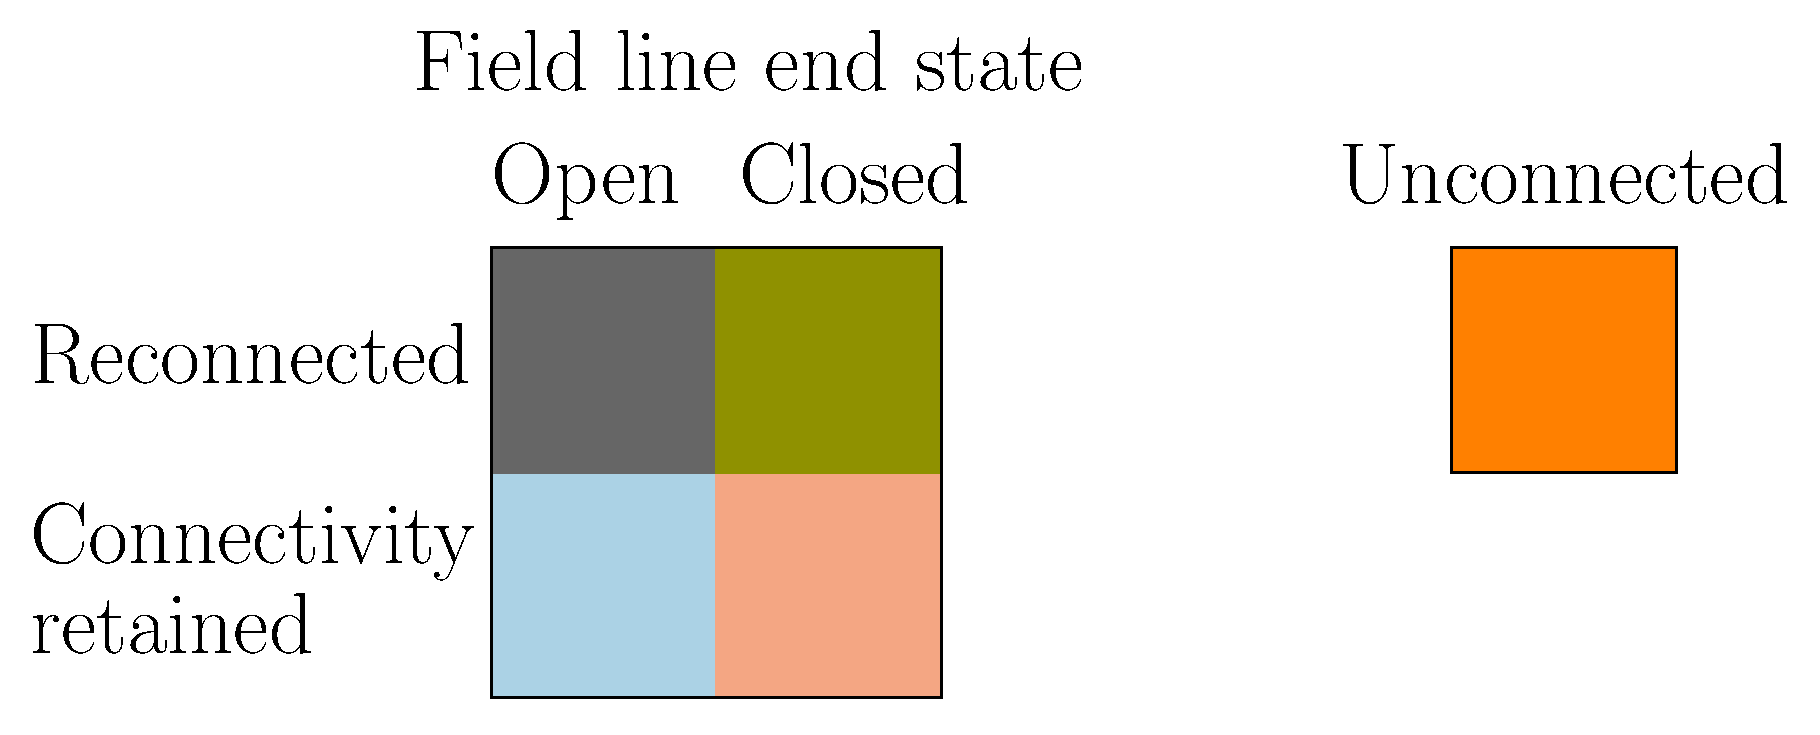
\includegraphics[scale=0.3]{Connectivity_Legend.pdf}

The two categories of reconnected field lines are determined by moving a cage of fieldlines and comparing the start and end connectivity at the cage location. For such a connectivity map to be constructed, \texttt{QSL Squasher} must be used to generate a minimum of two $Q$ maps for a comparison to be made. Once complete, modify the file \texttt{Connectivity\_Map\_Create.F90}, specifying \texttt{output\_times} using the method above, specify paths to \texttt{QSL\_files} and output paths to \texttt{connectivity\_files}. Once compiled, the program can be executed with

$\quad\quad$\texttt{./Connectivity\_Map\_Create}

This will take quite a while to run (currently not multithreaded). The connectivity files can then be displayed using \texttt{Plot\_Connectivity\_Map.py} or \texttt{Animate\_Connectivity\_Map.py}.


\end{document}
